\section{Performance Optimization}\label{sec:backend_optimization}

To ensure low-latency responses for the frontend, the backend implements a
Redis-based caching strategy using a dedicated \texttt{cacheHelper} middleware.
This caching layer intercepts all FHIR resource requests and serves repeated
reads directly from memory, substantially reducing load on the FHIR server and
PostgreSQL database.

\begin{figure}[H]
    \centering
    \fbox{\begin{minipage}{\dimexpr\textwidth-2\fboxsep-2\fboxrule\relax}
            \centering
            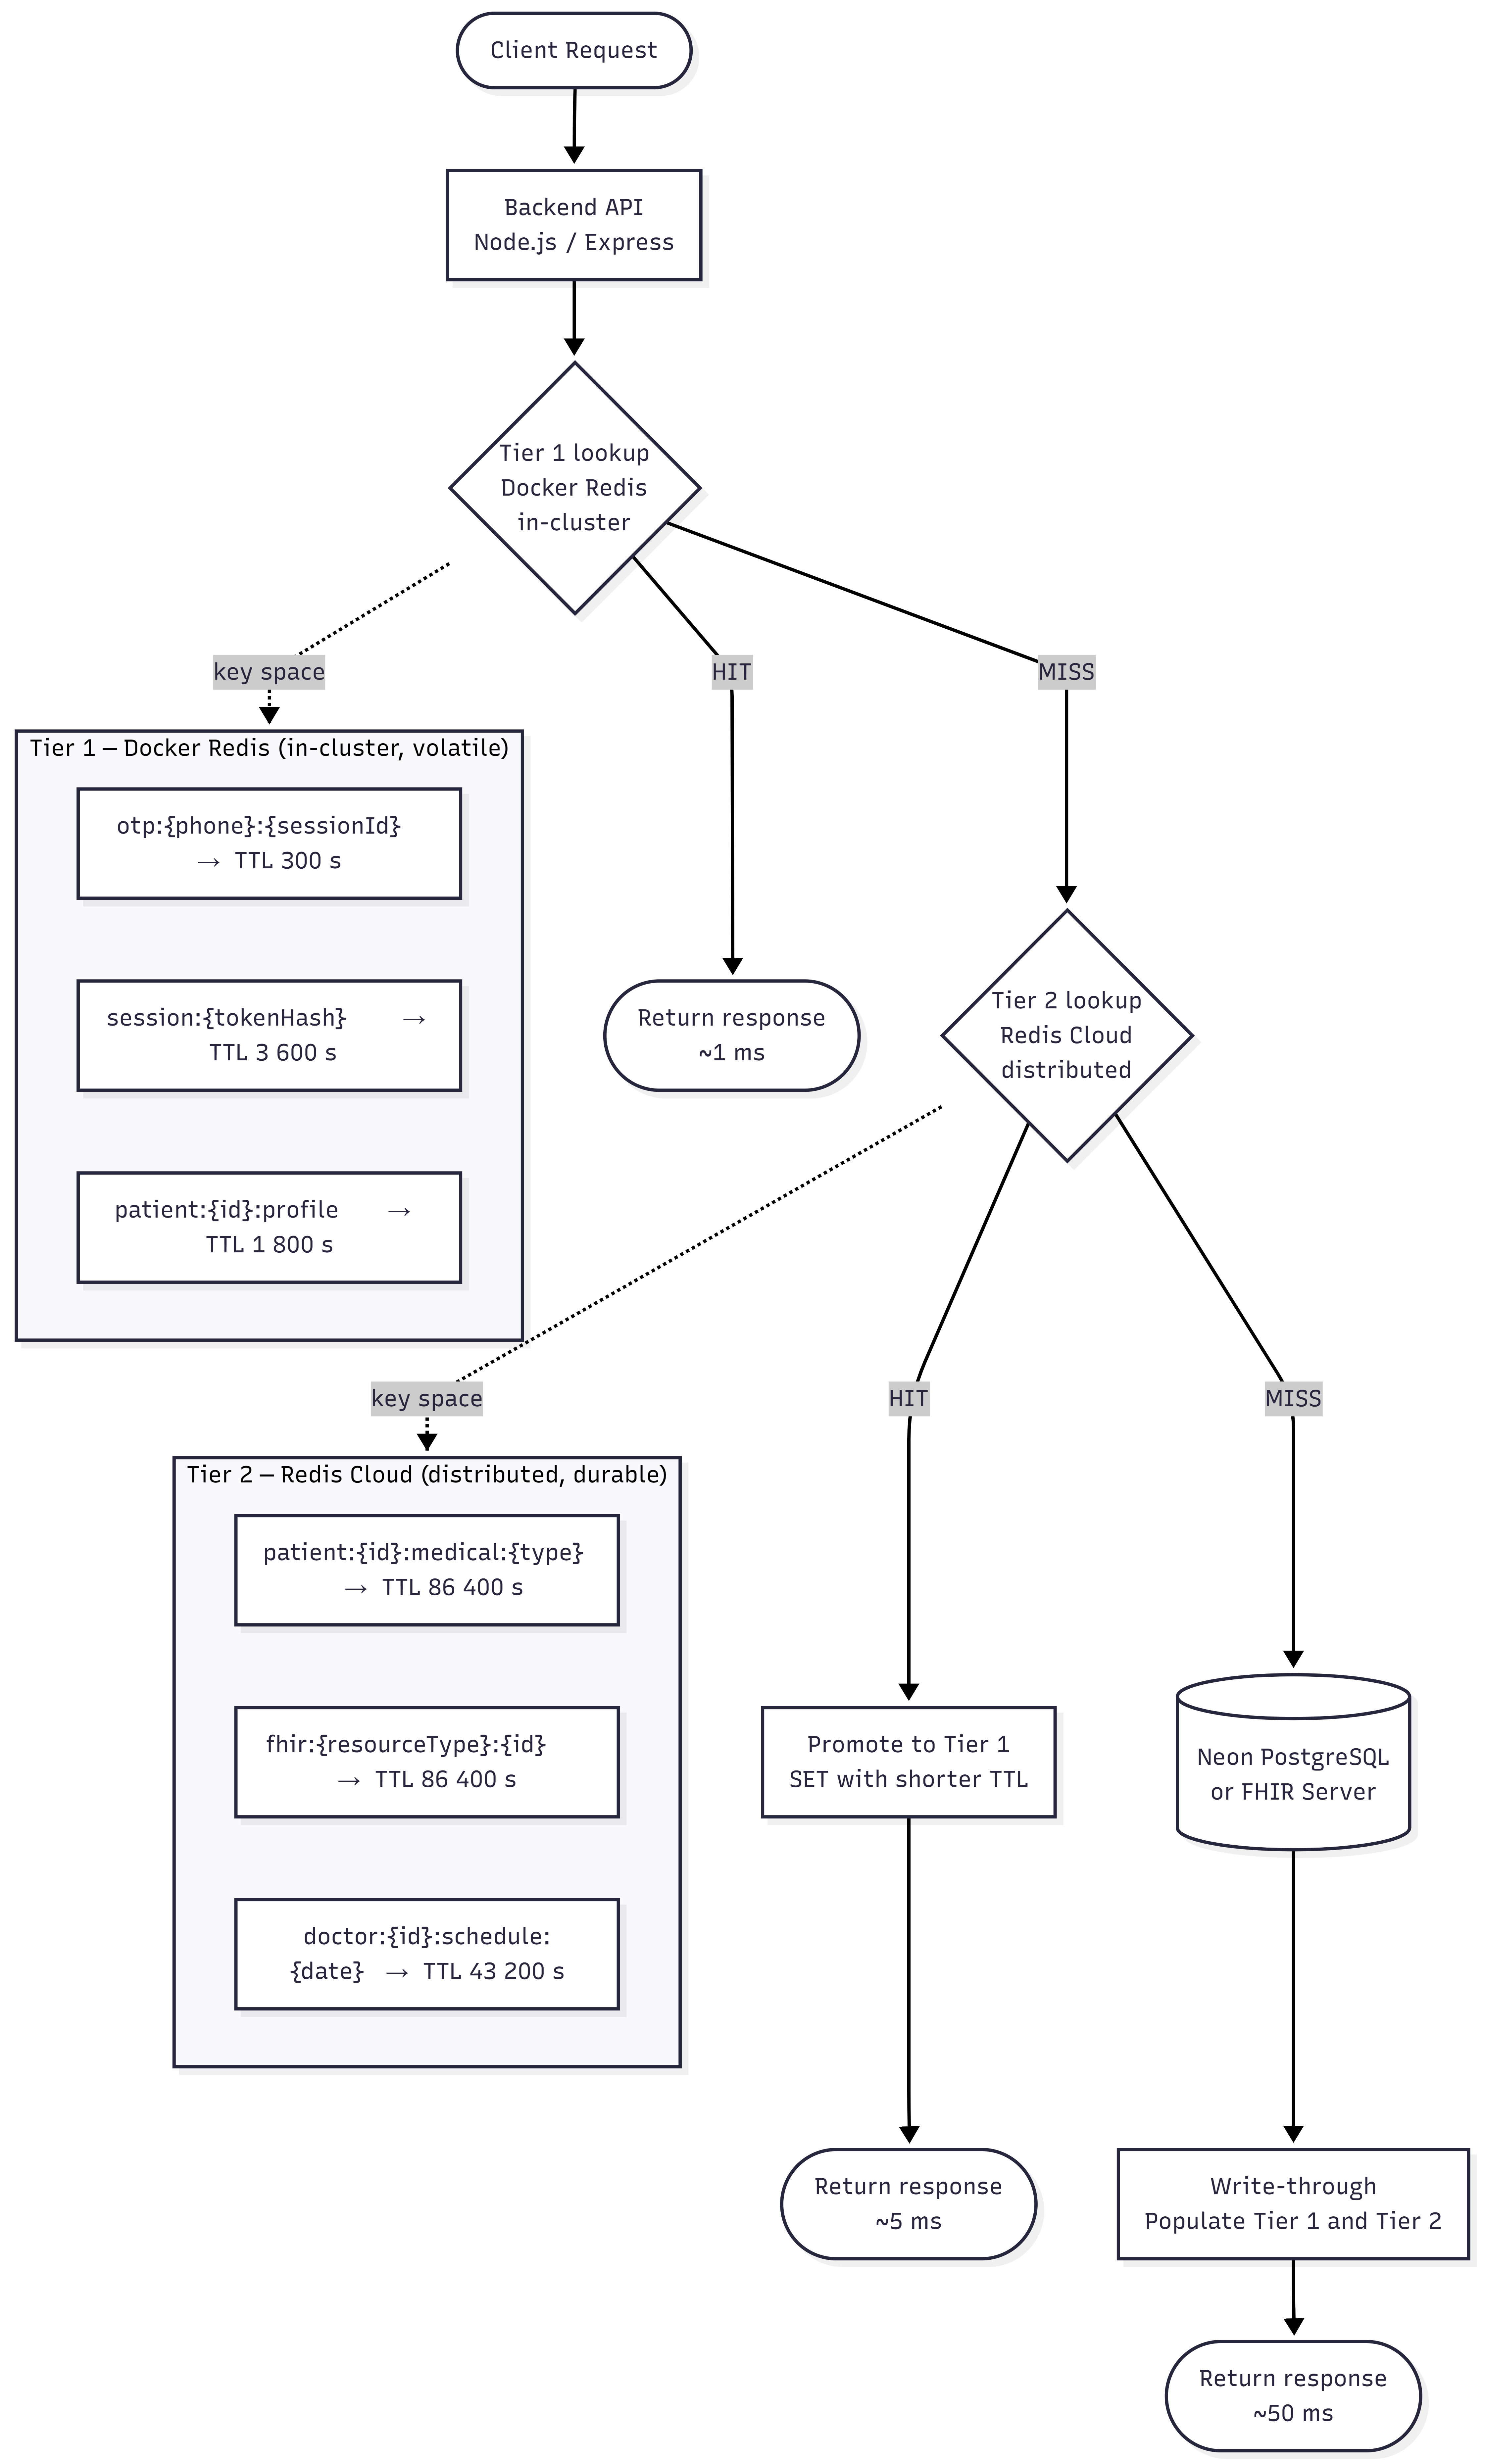
\includegraphics[width=0.9\linewidth]{Backend/Images/cachingGraph.png}
        \end{minipage}}
    \caption[Redis Caching Architecture]{Redis Caching Architecture showing the request flow through the \texttt{cacheHelper} middleware, cache hit and miss paths, and write-triggered invalidation.}\label{fig:caching}
\end{figure}

\subsection{Resource Cache}\label{subsec:resource_cache}

The backend utilizes a generic \texttt{cacheHelper} middleware that
intercepts HTTPS requests for standard FHIR resources. This middleware operates
at the request level, functioning as a transparent cache layer between the
frontend client and the backend processing pipeline.

\subsubsection{Mechanism and Interception}
When an HTTPS request arrives at the backend (such as a GET request to
\texttt{/api/patients}), the \texttt{cacheHelper} middleware performs a
sequence of operations to determine whether a cached response can be served.
The middleware first generates a deterministic cache key from the request URL
and query parameters---for example, a request to
\texttt{/api/patients?page=1\&{}limit=20} generates the key
\newline\texttt{cache:patients:page:1:limit:20}. The middleware then queries the Redis
cache for an entry matching this key. If a valid cache entry exists, meaning
the entry has not expired, the cached response is immediately returned to the
client, entirely bypassing the FHIR server, database query execution, and all
downstream processing. This direct cache-to-client path reduces latency from
potentially 500--2000ms (database query time) to sub-50ms (Redis in-memory
retrieval). If no entry exists or the entry has expired, the request proceeds
through the normal processing pipeline: the backend queries the FHIR server,
processes the response, and returns it to the client. Before returning, the
response is stored in Redis for future requests, repopulating the cache.

\subsubsection{Time-To-Live (TTL) Management}
Cached FHIR resources are assigned a uniform Time-To-Live (TTL) of
\textbf{60 seconds}. This short window ensures that data staleness never
exceeds one minute, which is clinically acceptable for the read-heavy
operations performed during active consultations. From a system load
perspective, the 60-second TTL substantially reduces the query volume to the
underlying FHIR server and database during bursts of concurrent requests---for
example, when multiple clinicians access the same patient record within the
same minute. The 60-second TTL applies uniformly across all resource types
including patients, conditions, encounters, medications, procedures, and
history graph entries.

\subsubsection{Cache Invalidation}
In addition to TTL expiration, certain write operations trigger explicit cache
invalidation immediately to ensure data consistency. When a patient record is
modified---such as contact information changes or new allergies being
recorded---the corresponding cache entries for that patient are removed,
forcing a fresh fetch on the next request. When a new encounter is recorded or
an existing one is updated, all cache entries scoped to that patient
(e.g.\ \texttt{patient:\{id\}:*}, \texttt{encounters:patient:\{id\}},
\texttt{historyGraph:patient:\{id\}:*}) are invalidated simultaneously. The
system maintains a dependency mapping between cache key namespaces and their
associated FHIR resources, ensuring that no stale references persist across
related endpoints after a write.

\subsubsection{Practical Impact}
The benefit of caching is most apparent during bursts of concurrent reads
within the same 60-second window. Without caching, every request triggers a
FHIR server round-trip costing 500--2000ms. With the cache populated, repeated
reads within the same minute are served from Redis in sub-50ms, a latency
reduction of one to two orders of magnitude. For example, when multiple
clinicians view the same patient's dashboard simultaneously, only the first
request incurs the full FHIR query cost; all subsequent requests within that
minute are served from memory. Beyond the 60-second TTL, write-triggered
invalidation ensures that any update to a patient's record is reflected on the
next request regardless of where the TTL stands, keeping the system consistent
without requiring manual cache management.

\subsubsection{Memory Management and Cache Eviction}
Redis is configured with a maximum memory limit to prevent unbounded growth and
to integrate into production server resource constraints. To manage memory
efficiently, the CFI-Care backend employs an LRU (Least Recently Used) eviction
policy. When Redis approaches its configured maximum memory capacity, the
system automatically evicts the least recently accessed cache entries to make
space for new data. This dynamic approach to cache management creates a natural
working set where the cache automatically retains entries for patients with
active clinical workflows (frequently accessed by multiple clinicians) while
entries for inactive patients are evicted and subsequently reconstructed
on-demand if and when those patients are accessed again. This ensures that
memory usage remains bounded and predictable while simultaneously maximizing
cache hit rates for the active subset of patients. In practice, this means that
high-volume clinical workflows benefit from maximum cache coverage, while less
frequently accessed patients gracefully degrade to on-demand reconstruction
without requiring administrator intervention or manual cache management.
